\section{Preliminaries on the Dual View for DNN with ReLUs}\label{sec:prelim}
In this section, we make a brief presentation of the preliminaries dual view formulation for a fully connected (FC) DNN with ReLUs in \citep{npk}. We consider a FC-DNN with `$d$' layers and  $w$  hidden units in each layer. The quantites `path feature' and `path value' in \Cref{sec:intro} will henceforth be called as \emph{neural path feature}(NPF) and \emph{neural path value} (NPV); these are defined in \Cref{def:npf-npv}. \Cref{prop:npf-npv} show that the output is the inner product of the NPF and NPV. \Cref{lm:npk} shows the relationship between the \emph{neural path kernel} (NPK), the Gram matrix of the NPFs, and a correlation matrix capturing subnetwork overlaps. 

\begin{definition}\label{def:npf-npv}
A path starts from an input node, passes through a weight and a hidden unit in each layer and ends at the output node. We define the following quantities for a path $p$:
\emph{
\begin{tabular}{lcl}
 Activity&:& $A_{\Theta}(x,p)$ is the product of the `$d-1$' gates in the path. \\
Value&:& $v_{\Theta}(p)$ is the product of the `$d$' weights in the path.\\
Feature&:&   $\phi_{\Theta}(x,p)$ is the product of the signal at the input node of the path and $A_{\Theta}(x,p)$.\\
\end{tabular}
}

The \emph{neural path feature} (NPF) given by $\phi_{\Theta}(x)=\left(\phi_{\Theta}(x,p),p=1,\ldots, \Pfc\right),\in\R^{\Pfc}$ and the \emph{neural path value} (NPV) given by $v_{\Theta}=\left(v_{\Theta}(p),p=1,\ldots,\Pfc\right),\in\R^{\Pfc}$.
\end{definition}

\begin{proposition}\label{prop:npf-npv}
The output of the DNN is then the inner product of the NPF and NPV: 
\begin{align}\label{eq:inner}
\hat{y}_{\Theta}(x)=\ip{\phi_{\Theta}(x),v_{\Theta}}=\sum_{p\in[P]}  \phi_{\Theta}(x,p) v_{\Theta}(p)
\end{align}
\end{proposition}
\begin{figure}[t]
\centering
\resizebox{0.9\columnwidth}{!}{
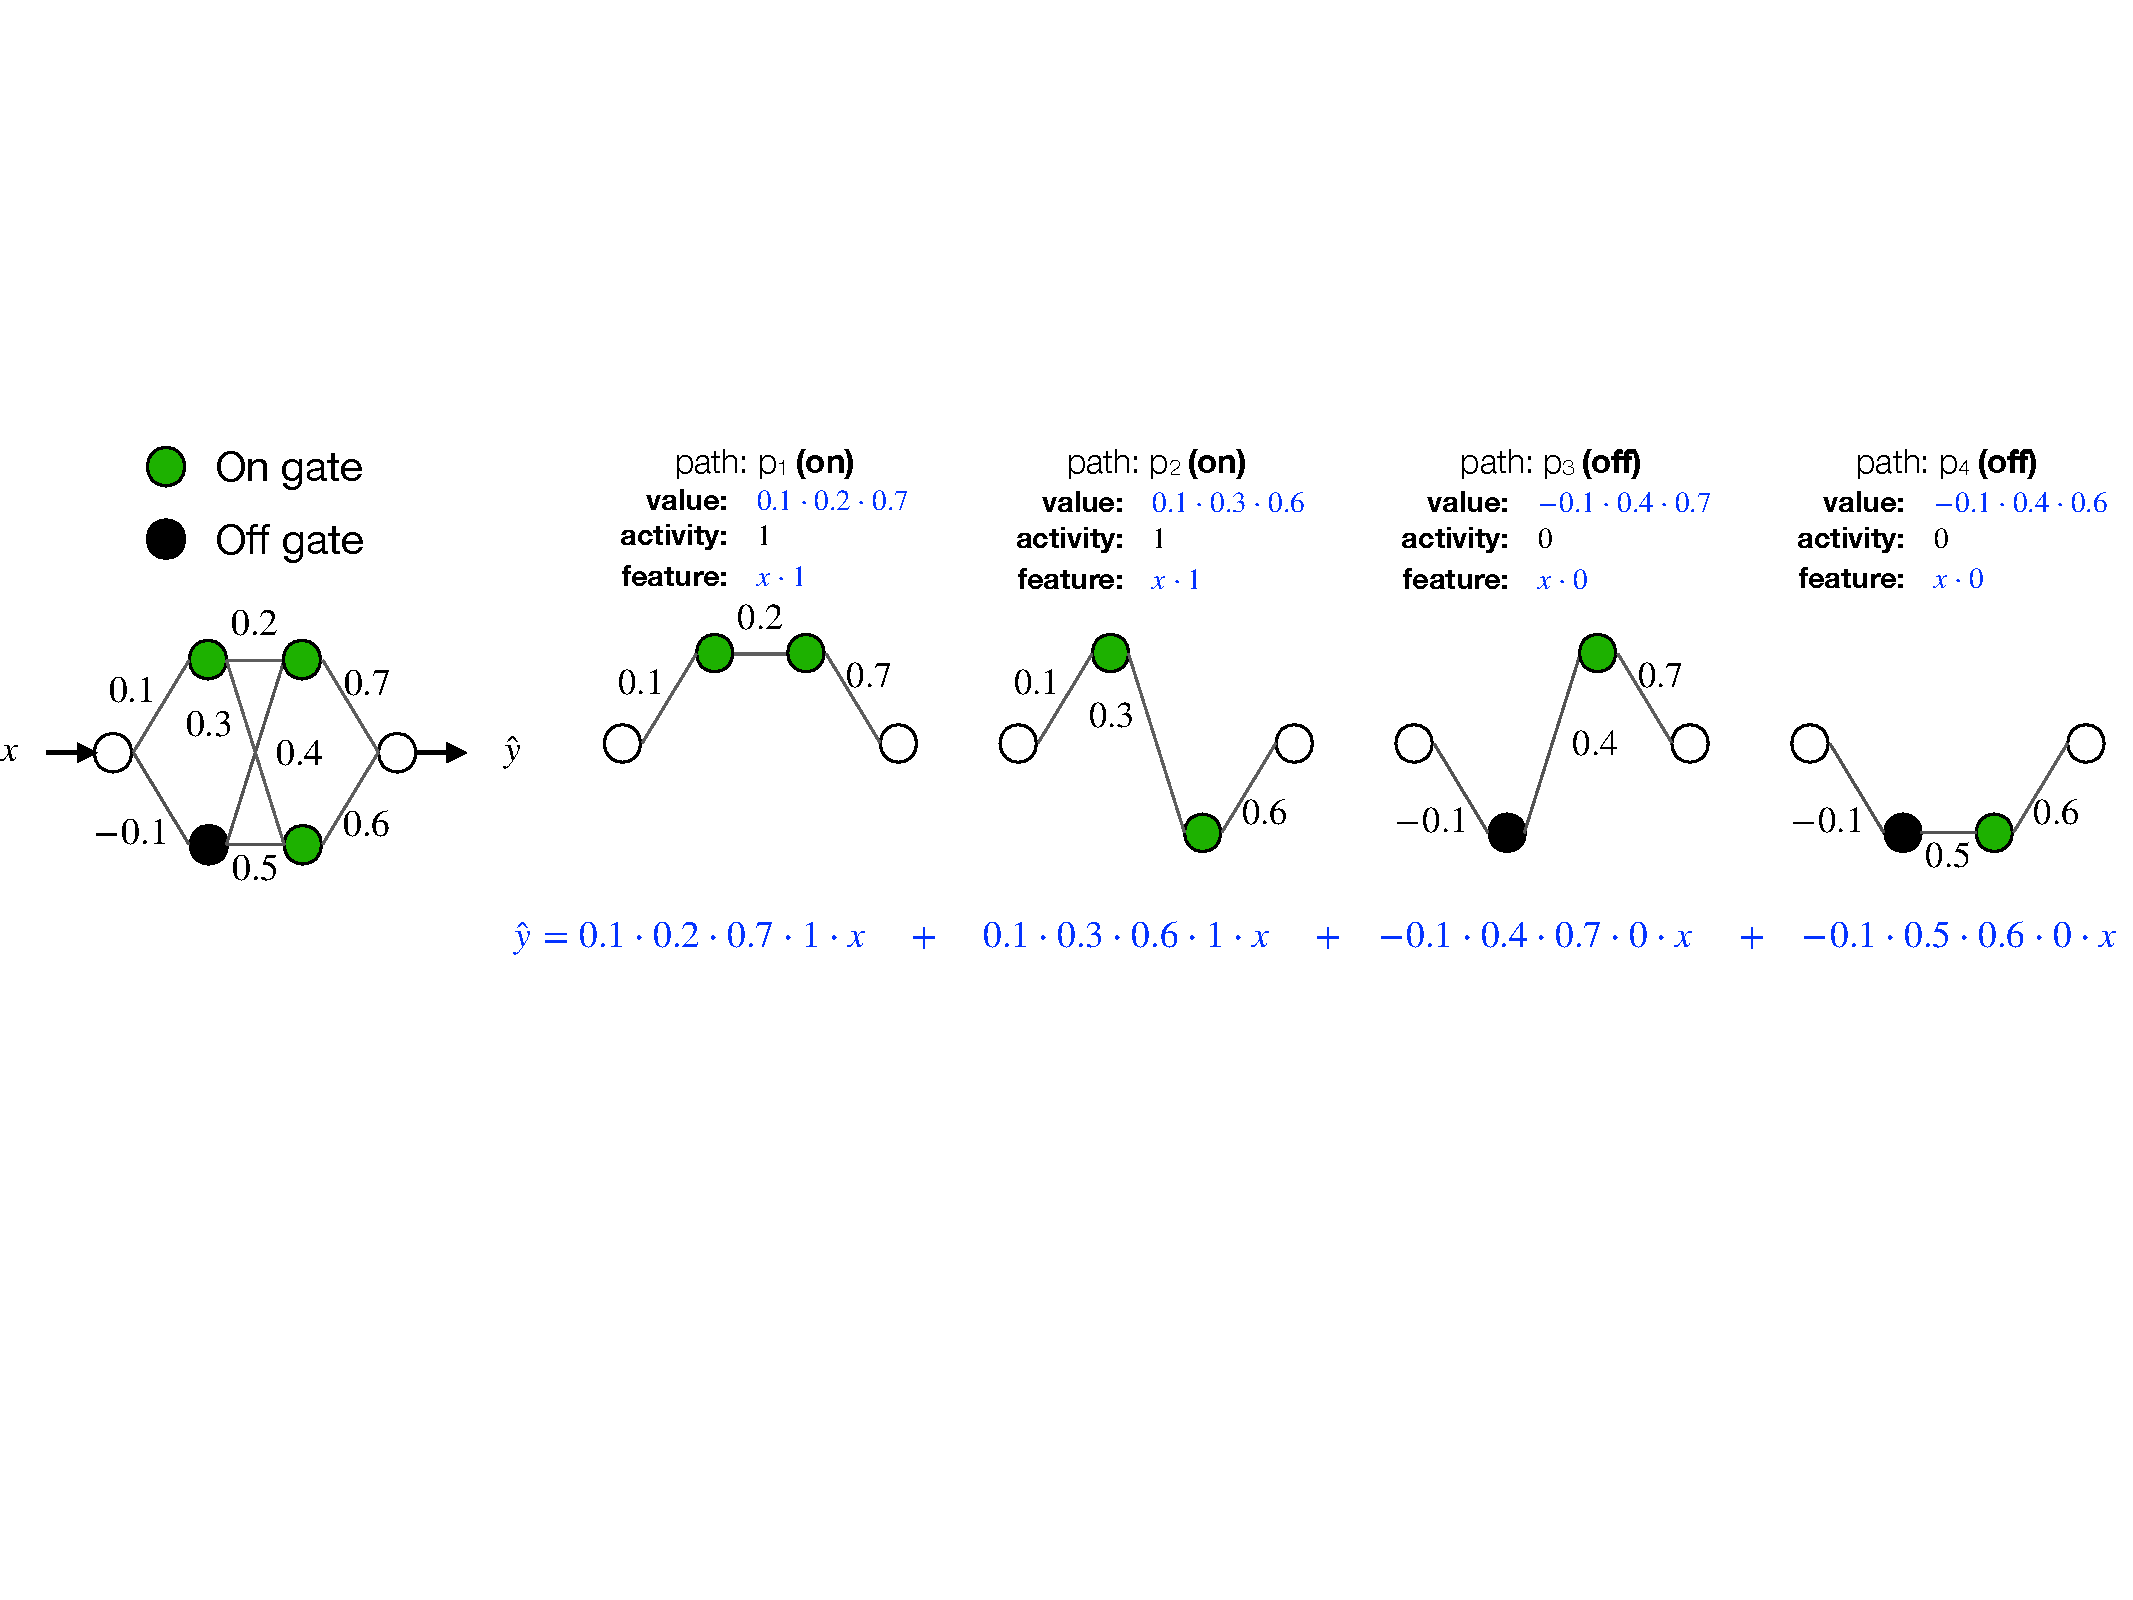
\includegraphics[scale=0.5]{figs/paths.pdf}
}
\caption{Illustration of \Cref{def:npf-npv} and \Cref{prop:npf-npv} in a  toy network with $2$ layers, $2$ gates per layer and $4$ paths. Paths $p_1$ and $p_2$ are `on' and paths $p_3$ and $p_4$ are `off'. The value, activity and feature of the individual paths are shown. $\hat{y}$ is the summation of the individual path contributions.}
\label{fig:paths}
\end{figure}

%\subsection{Overlap of Sub-Networks and Neural Path Kernel}
\begin{definition}[Overlap of active sub-networks]\label{def:overlap} 
The total number of `active' paths for both $x$ and $x'$ that pass through input node $i$ is defined to be:\\
{\centering{\centering{$\textbf{overlap}_{\Theta}(i,x,x') = \Lambda_{\Theta}(i,x,x') \eqdef \left|\{p \colon  A_{\Theta}(x,p)= A_{\Theta}(x',p)=1\}\right|/\din$}}}
\end{definition}
%\subsection{NPK of FC-DNN: Product Kernel }
%\input{cnpkexample}
%\subsection{Neural Path Kernel : Similarity based on active sub-networks}
\begin{lemma}[Neural Path Kernel (NPK)]\label{lm:npk}
Let $D\in\R^{\din}$ be a vector of non-negative entries  and for $u,u'\in\R^{\din}$ , let $\ip{u,u'}_{D}=\sum_{i=1}^{\din}D(i)u(i)u'(i)$. Let $H_{\Theta}(x,x')\eqdef\langle\phi_{\Theta}(x),\phi_{\Theta}(x') \rangle$ be the neural path kernel (NPK). Then  
\begin{align*} 
\text{NPK}_{\Theta}(x,x')= H_{\Theta}(x,x')=\ip{x,x'}_{\Lambda_{\Theta}(\cdot,x,x')} 
\end{align*}
\end{lemma}
\textbf{Remark.} In the case of fully connected networks, $\textbf{overlap}_{\Theta}(i,x,x')$ is equal for all $i\in[\din]$, and hence $\text{NPK}_{\Theta}(x,x')=\ip{x,x'}\cdot\textbf{overlap}_{\Theta}(x,x')$.

